\documentclass{article}
\begin{document}
%===========================
%===========================
%===========================
\section{Introduction}

%===========================
%===========================
%===========================
\section{Experimental setup}
%=========
\begin{figure}
  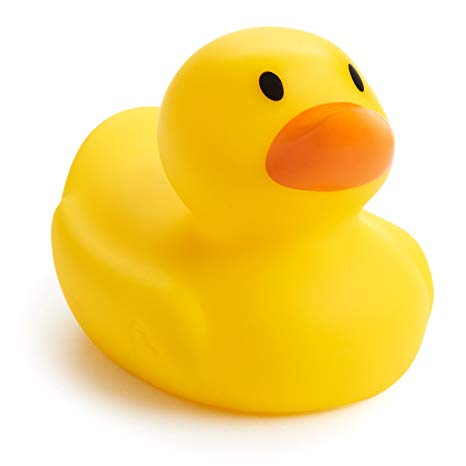
\includegraphics[width=0.8\textwidth]{temp.jpg}
  \label{Chemically etched boards and chamber installation}
\end{figure}
%=========
\begin{figure}
  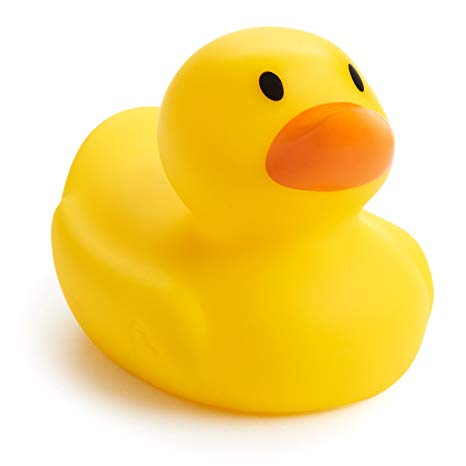
\includegraphics[width=0.8\textwidth]{temp.jpg}
  \label{Configuration of chambers with different avalanche techniques}
\end{figure}

%===========================
%===========================
%===========================
\section{Data analysis}
%=========
\begin{figure}
  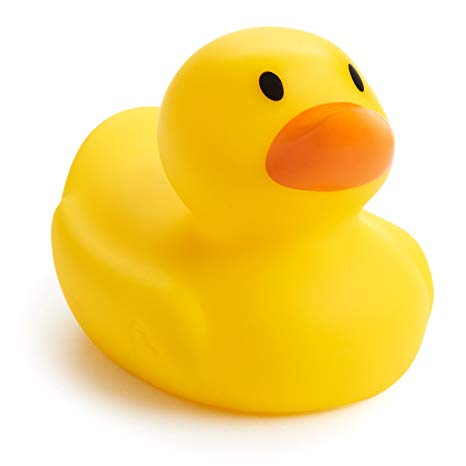
\includegraphics[width=0.8\textwidth]{temp.jpg}
  \label{Comparison of cluster widths for typical response of each avalanche technology under normal running configurations.}
\end{figure}
%=========
\begin{figure}
  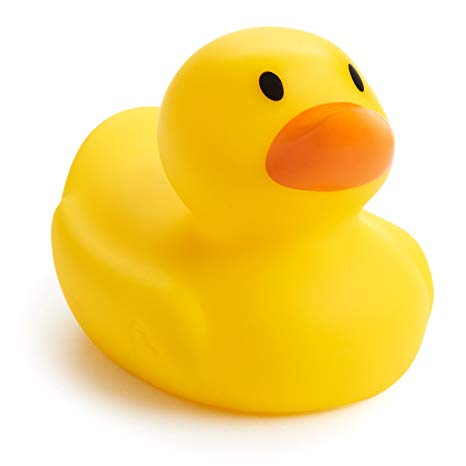
\includegraphics[width=0.8\textwidth]{temp.jpg}
  \label{Example of 2D-correction due to differential non-linearity.}
\end{figure}

%===========================
%===========================
%===========================
\section{Results}
%=========
\begin{figure}
  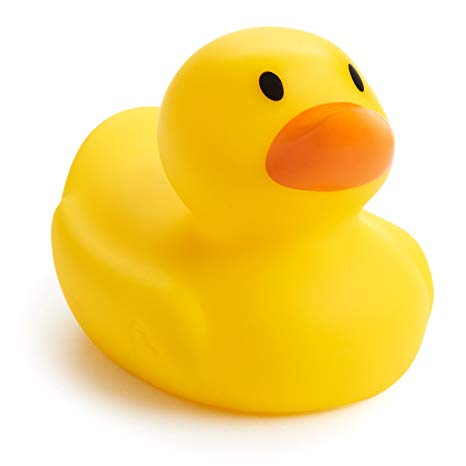
\includegraphics[width=0.8\textwidth]{temp.jpg}
  \label{Coparison of resolution as a function of X-stretch (\%) for a particular X-pitch and Y-period configuration.}
\end{figure}
%=========
\begin{figure}
  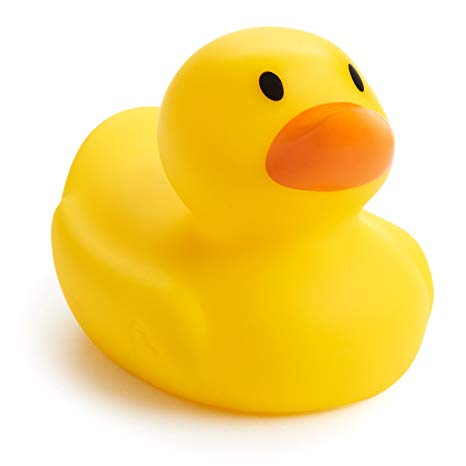
\includegraphics[width=0.8\textwidth]{temp.jpg}
  \label{Coparison of resolution as a function of X-pitch (\%) for a particular X-stretch and Y-period configuration.}
\end{figure}

\section{Discussion}
\end{document}
